\documentclass[titlepage]{article}

\usepackage{cite}
\usepackage{graphicx}
\graphicspath{ {images/} }
\usepackage{caption}
\usepackage[]{appendix}
\usepackage{multicol}
\usepackage{listings}

\setlength{\columnseprule}{1pt}


\begin{document}
\title{EGH456: Embedded Systems \\ Motor Controller for Electric Vehicles}

\author{\parbox{\textwidth}{\begin{multicols}{2}\begin{flushright}
Daniel Huffer \\ 
Mitchell Bourne \\ 
Wu Jason \\ 
Zachary Hugo
\end{flushright}\columnbreak\begin{flushleft}
nXXXXXXX \\ 
nXXXXXXX \\ 
nXXXXXXX \\ 
n9158332
\end{flushleft}\end{multicols}}}

\maketitle



\begin{abstract}
\end{abstract}

\tableofcontents
\listoffigures
\listoftables
\clearpage


\section{Introduction}
Introduction – Problem statement, context, requirements, and statements on the individual
contributions by each team member. (2 pages)



\section{Design and Implementation}
– Approach to design, important issues and choices and their
relationships to theoretical concepts and the hardware and software platforms. Check if you
have addressed:
◦ Provided a graphical representation for your design?
◦ Provided a Project Folders and Files diagram?
◦ Did you use the GPIO module? How? Did you use the graphics library? How? Did you
use Tasks, Hwi and Swi? How?
◦ Did you use multiple threads/handlers? How? Did you use the ADC? How?


\section{Design Notes (Zachs bullshit)}
\begin{figure}[h]
\caption{Motor Control Schematic}
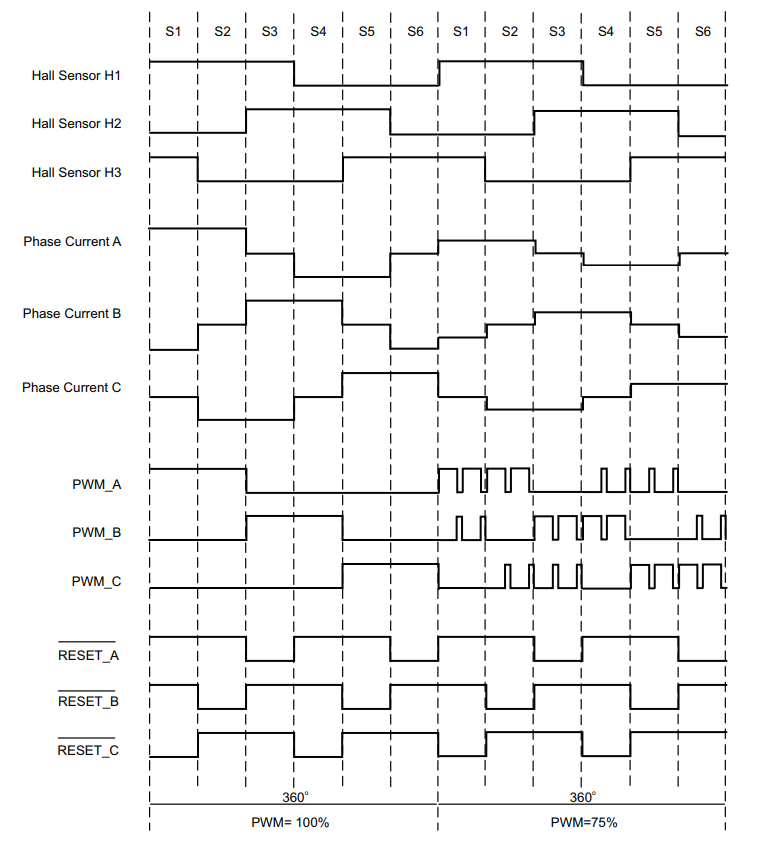
\includegraphics[scale=0.4]{motor_order.png}
\end{figure}
%Add source from data sheet

3 GPIO in for the hall effect sensors\\
3 timers set in PWM mode, corresponding to 3 motor pins\\
3 GPIO out for motor driver reset

Motor power is set by a PWM value.\\
Value determined by PI controller (one line of code)\\
Maybe make a set power and target power, and limit the rate of change of the set power until it gets to the correct output. This may reduce the amount of stuff we need in a start up function. Not sure if it will affect controller too much.


Hall effect sensors measure motor position. The order that the hall effect sensors turn high gives motor direction. \\
Hwi called each time sensor goes high.

Calls a single Swi with an argument saying what hall effect sensor called it\\
Swi sets the PWM duty cycle of one motor phase to the one determined by the PI controller. Others set to 0. Resets also set. 

Things to consider: The motor control schematic shows that other coils are energised with the inverse of the pwm signal at 180 degrees out of phase. We can get away without this for now.

This assumes that the hall effect sensor is correctly aligned with the motor. The assignment calls for special features. We can adjust the timing by adding a one shot timer before the SWI is called (maybe). We can also show that a timing is optimal if the steady state current is as low as it can be. Auto tune function should be doable if we get time. 

We may also want to consider a timer based system that subdivides the time between pulses. This will allow us to ramp up the voltages closer to a sin wave. Might be more efficient and something to write about to get a 7



\clearpage
\begin{lstlisting}
sudo code

hwi hf1() { 
	motor_swi(1);
}

hwi hf2() {
	motor_swi(2);
}

hwi hf3() {
	motor_swi(3);
}

swi motor_swi(int hf) {
	for(int i = 0; i < 3; i++) {
		if(hf == i) {
			motor(i) = power;
		} else {
			motor(i) = 0;
		}
	}
}

% call this around 100hz / every 10ms
timer_interrupt power{
	Kp = n; %Proportional coefficient
	Ki = n; %Integral coefficient

	error = desired_speed - actual_speed;
	
	cum_error += error
	
	if (cum_error > limit) {cum_error = limit};

	desired_power = Kp*error + Ki * cum_error;

	% control rate, not sure if needed. 
	% Maybe just put in separate soft start function in startup
	if(set_power > desired power) {
		set_power -= 0.01 * max power
	} else if (set_power < desired power) {
		set_power += 0.01 * max power
	}
}




\end{lstlisting}


\section{Results}
Summary of evidence of functional requirements that were demonstrated and
explanation of failures as learning outcomes in terms of what could have been done
differently. (2 pages)















\clearpage
\addappheadtotoc
\appendixpage
\appendix
Mention the name of the hardware development platform and versions of the
tools used such as Code Composer Studio, Tivaware, TI-RTOS, etc. (1 page)


\clearpage
\addcontentsline{toc}{section}{References}
\begin{thebibliography}{9}
Including vendor supplied technical documents with a table that links each
document to sub-sections of your report where they are relevant with entries: The reference
number, the sub-section number, topic keyword or keywords, the pages that were found
useful. (2 pages)

\end{thebibliography}
\end{document}
